\section{The ResNet}
\label{sec:resnet}

The \emph{Residual Network (ResNet)} is a deep neural network architecture first introduced by \Citeauthor{heDeepResidualLearning2015}\cite{heDeepResidualLearning2015} in 2015, which addresses the seemingly paradoxical circumstance that adding more layers to a deep neural network would degrade its performance compared to a shallower network, even though the solution space of the shallower model is a subspace of its deeper counterpart. 

Working from the idea that adding more layers to a network should not produce a higher error, since the additional layers could potentially just learn identity mappings, the authors surmised that the problem lied with the difficulty for the optimization process to learn the underlying desired mapping for a set of layers if the ideal mapping is closer to an identity mapping than a zero mapping.

The solution to this, proposed by ResNet, is to utilize residual connections between the input and output of a layer group, by directly adding the input to the output. 
Instead of having to learn the desired output mapping $\mathcal{H}(x)$, the layers now have to fit the residual mapping $\mathcal{F}(x) := \mathcal{H}(x) - x$, which the authors argue is easier for the optimizer to do.

\begin{figure}[htbp]
    \makebox[\textwidth][c]{
        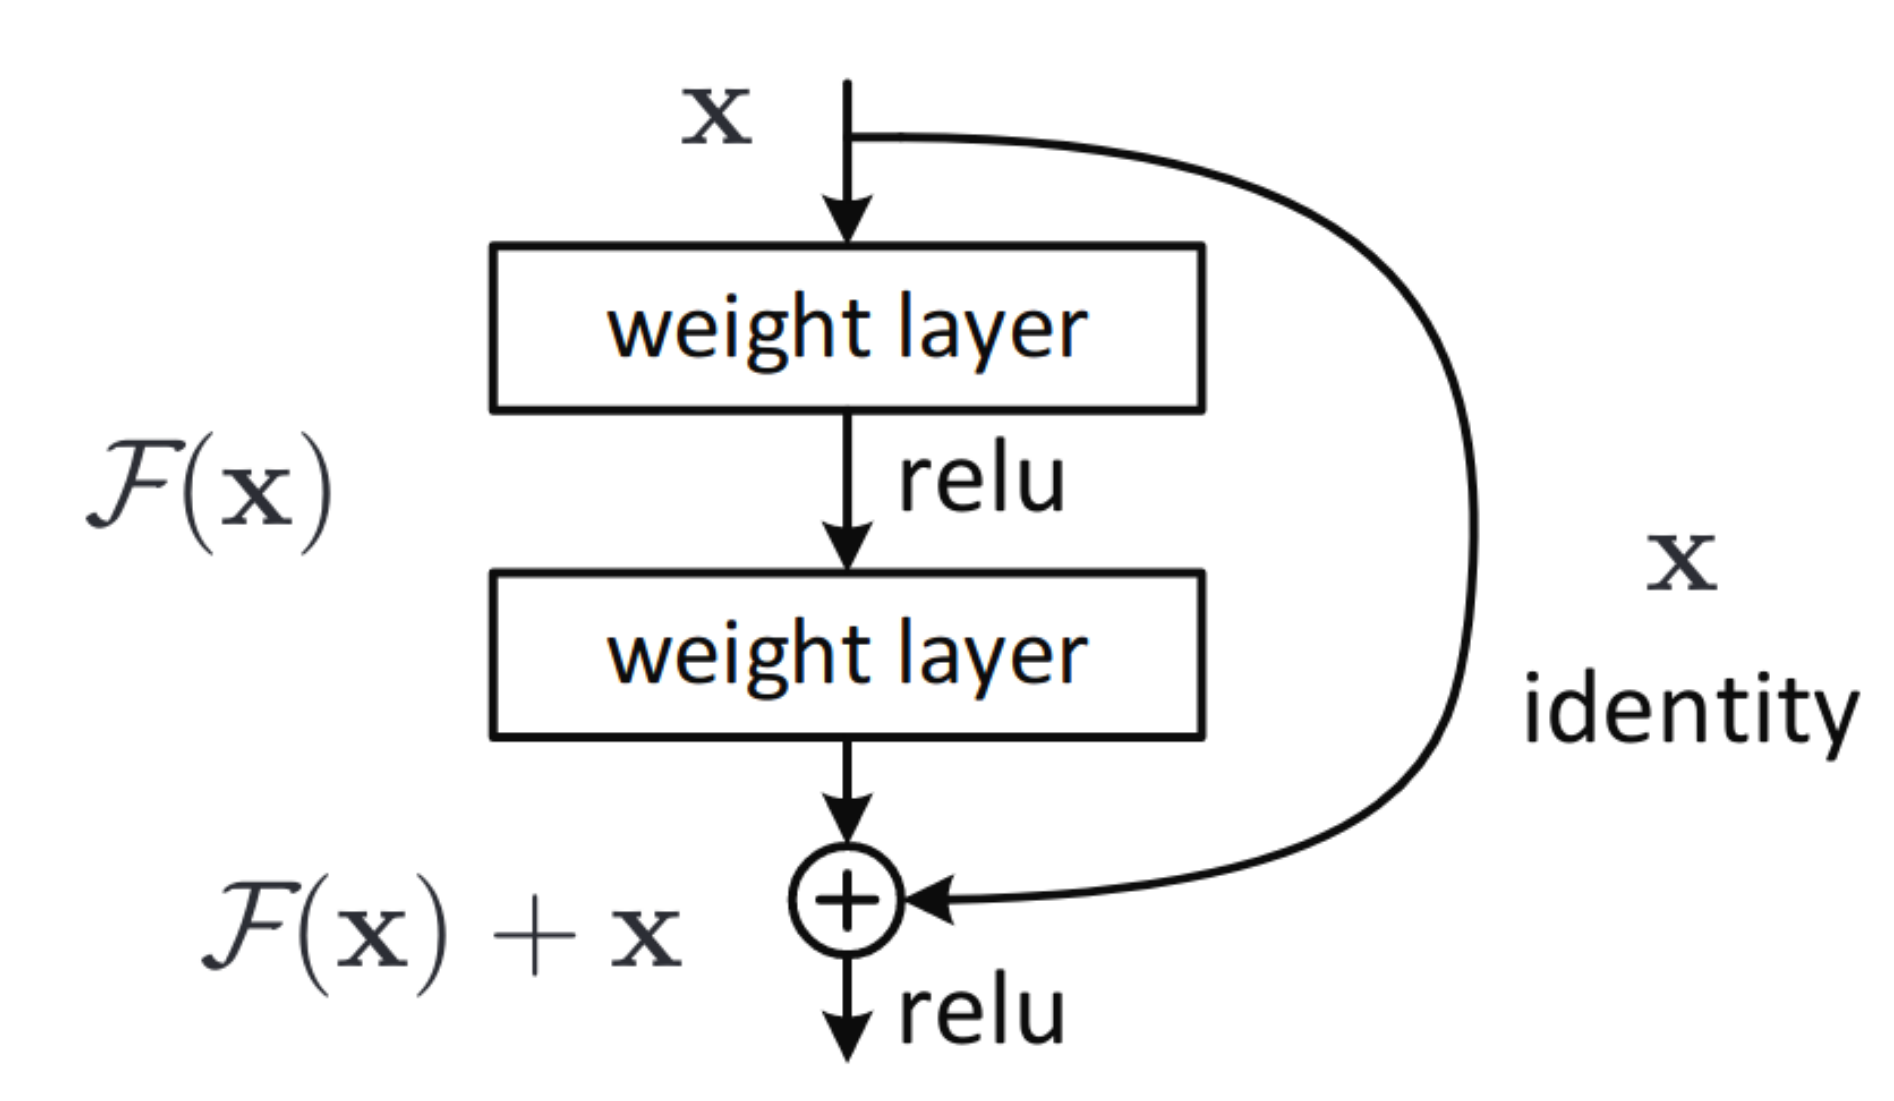
\includegraphics[width=0.4\textwidth]{images/Screenshot-20230207134546-1894x1101.png}
    }
    \caption{A depiction of a \emph{residual block} employed in the ResNet network architecture. The input of a group consisting of several layers is added directly to the output. The weighted layers can be linear layers but in practice, mostly convolutional layers are used. The blocks also consist of 3 layers the majority of the time. Image taken from \cite{heDeepResidualLearning2015}}
    \label{fig:resblock}
\end{figure}

Employing these \emph{residual blocks}, the convergence rate of the network is significantly improved, without adding any computational complexity. 
This enables the use of very deep networks, gaining substantial accuracy from the added layers.

Apart from the residual connections, the ResNet still follows a typical encoder architecture, with each block reducing spatial resolution, while increasing the number of feature channels.
There are several versions of the ResNet architecture, differing mainly by the number of layers used. 
\Citeauthor{heDeepResidualLearning2015} looks at networks with up to 152 layers (ResNet152), but deeper networks have been explored. 

Since the residual connection allow the network to propagate information from the shallower layers to the deeper layers more easily, it may also combat the problem of vanishing/exploding gradients, which were a challenge for increasingly deep models at the time, however the authors argue that this was already sufficiently addressed by regularization techniques such a \emph{Batch Normalization}. \cite{ioffeBatchNormalizationAccelerating2015}

ResNet was able to significantly outperform its state-the-art predecessors at the task of image classification and is widely used today, often as part of a larger model ensemble.

In this thesis, \emph{ResNet34 D} is used in most experiments, which makes several minor improvements over the regular ResNet.
This includes employing an average pooling layer before the strided $1\times 1$ convolution present in the identity path of each downsampling block to include all datapoints, switching the stride of convolutions in the residual path for the same reason and replacing the $7\times 7$ initial downsampling convolution with three $3\times 3$ convolutions.
These modifications see an improvement in classification error while only increasing computational cost slightly. \cite{heBagTricksImage2018} 

\begin{figure}[htbp]
    \makebox[\textwidth][c]{
        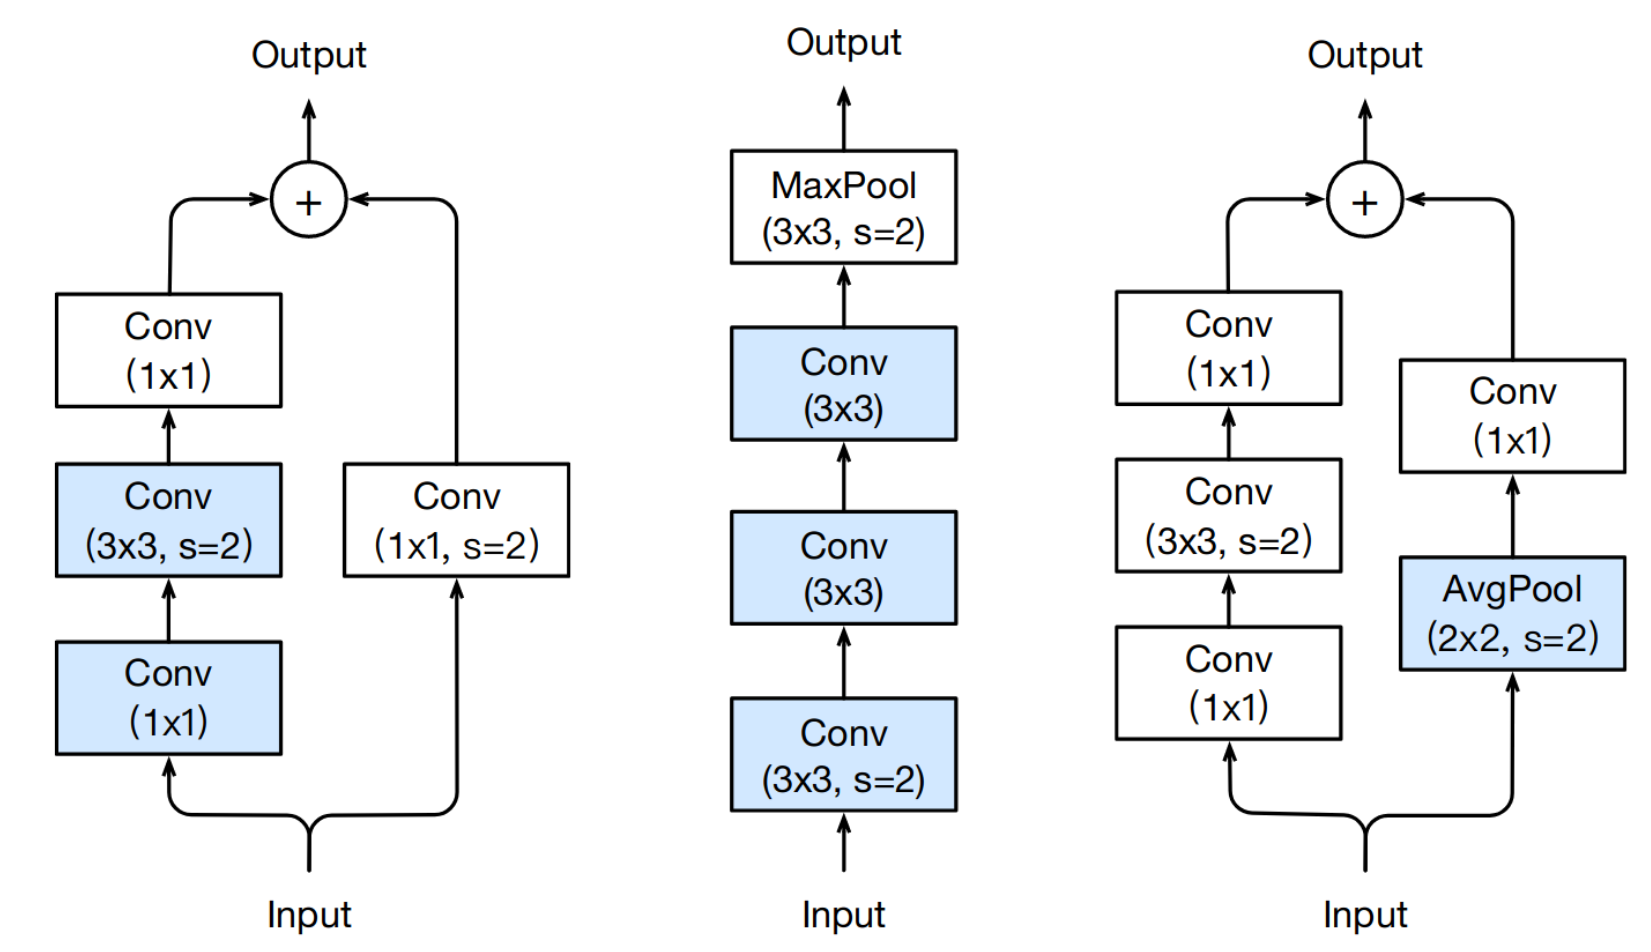
\includegraphics[width=0.9\textwidth]{images/Screenshot-20230207145624-1651x952.png}
    }
    \caption{Illustration of the three improvements made by ResNet34 D, with the blue boxes representing the changes made. Left depicts the change made to the residual path of the downsampling block, middle illustrates the changes made to the initial block of the network and right explains the changes to the identity path. $s$ represents the stride of the operations, with it being one if ommited. Image taken from \cite{heBagTricksImage2018}}
    \label{fig:resnet34d}
\end{figure}

\begin{figure}[htbp]
    \makebox[\textwidth][c]{
        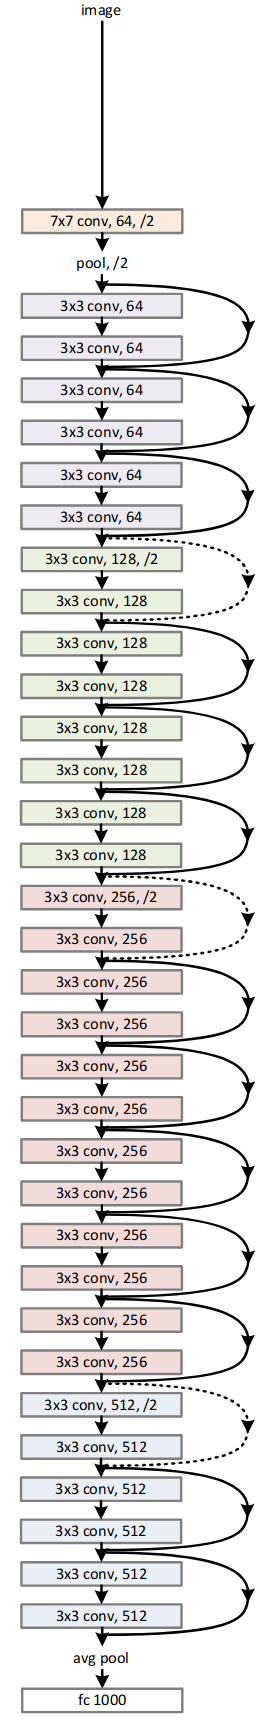
\includegraphics[width=0.2\textwidth]{images/Screenshot-20230207144959-265x1725.png}
    }
    \caption{Diagram for the ResNet34 model. Curved arrows represent a residual connection, with dotted arrows meaning the connection also downsamples the input. The four encoder blocks are colored differently. For use as an encoder, the fully connected layer at the end is omitted. Image taken from \cite{heDeepResidualLearning2015}}
    \label{fig:resnet34}
\end{figure}